%
% Angepasste FOM Seminarvorlage (2024)
%
\documentclass[12pt,a4paper,listof=totoc,bibliography=totoc]{scrartcl}

\usepackage[english]{babel}			% englische Namen/Umlaute
\usepackage[utf8]{inputenc}	    	% Zeichensatzkodierung
\usepackage{silence}
 \WarningFilter{scrartcl}{Usage of package `fancyhdr'}
 \WarningFilter{scrartcl}{Usage of package `parskip'}
\usepackage{fancyhdr}
\usepackage{graphicx}               % Einbinden von Bildern
\usepackage[hidelinks]{hyperref}	% Klickbare Verweise und \autoref{label}
\usepackage[intoc]{nomencl}
\usepackage{setspace}
\usepackage{parskip}
\usepackage{caption}
\usepackage{float}
% \usepackage{listings}
\usepackage{geometry}
 \geometry{a4paper, left=40mm, right=20mm, top=40mm, bottom=20mm}
\renewcommand{\familydefault}{\sfdefault}
\renewcommand{\ttdefault}{pcr}
% \renewcommand{\lstlistlistingname}{List of Code Examples}
% \renewcommand{\lstlistingname}{Example}

%
%RStudio
%
\usepackage{color}
\usepackage{fancyvrb}
\usepackage{framed}
\DefineVerbatimEnvironment{Highlighting}{Verbatim}{commandchars=\\\{\}}
\definecolor{shadecolor}{RGB}{241,243,245}
\newenvironment{Shaded}{\begin{snugshade}}{\end{snugshade}}
\newcommand{\NormalTok}[1]{\textcolor[rgb]{0.00,0.23,0.31}{#1}}

% Bildueberschrift oben und rechtsbuendig
\captionsetup{labelfont=bf, textfont=bf}
\captionsetup{justification=raggedright,singlelinecheck=false}

% Blocksatz
\def\justify{%
  \rightskip=0pt
  \spaceskip=0pt
  \xspaceskip=0pt
  \relax
}

%
%	Hier werden Titel, Bearbeiter und das Datum eingetragen
%
\newcommand\svthema{Rancher CNI Usage Recommendation}
\newcommand\svperson{Christian Frank (\#473088)}
\newcommand\svdatum{\today}
\newcommand\lvname{Data Science \& Security Analytics}
\newcommand\lvtyp{SS 2024}
\newcommand\lvinst{FOM - Hochschule für Oekonomie \& Management}
\newcommand\lvbetr{Prof. Dr. Alexander Lutz}

\hypersetup{ % Thema und Author in die Meta-Daten der PDF
  pdftitle={\svthema}, 
  pdfauthor={Christian Frank},
  pdfsubject={Rancher CNI usage recommendation},
  pdfkeywords={Kubernetes, Traffic, Rancher, CNI, Throughput}
}

\begin{document}

% Titel
\title{ \huge\textbf{\svthema} }
\author{ {\svperson} \\ \svdatum }
\date{ \normalsize \centering 
\includegraphics[width=0.3\textwidth]{FOM}\\ {\lvname} \\ {\lvbetr} \\ {\lvinst} \\ {\lvtyp} }

% Seitennummer oben
\pagestyle{fancy}
\fancyhf{}
\fancyhf[ch]{\thepage}
\renewcommand\headrulewidth{0pt}

\maketitle
\thispagestyle{empty} % laesst die Seitennummer auf der Titelseite verschwinden
\pagenumbering{Roman}

\begin{abstract}
This paper will perform a secondary analysis of Kubernetes CNI performance data, focusing on the CNIs available in the Rancher Kubernetes Engine. It aims to make a usage recommendation.

\end{abstract}

\vfill
\begin{figure}[h]
    \centering
    
\includegraphics[]{CC-BY}
\end{figure}

This work is licensed under the Creative Commons Attribution 4.0 International License. To view a copy of this license, visit http://creativecommons.org/licenses/by/4.0/ or send a letter to Creative Commons, PO Box 1866, Mountain View, CA 94042, USA.

\cleardoublepage

\tableofcontents			% Inhaltsverzeichnis
\cleardoublepage

\listoffigures				% Abbildungsverzeichnis
\cleardoublepage

\listoftables               % Tabellen
\cleardoublepage

% \lstlistoflistings			% Codeverzeichnis
% \cleardoublepage

%
% Abkuerzungsverzeichnis
%
\makenomenclature
\renewcommand{\nomname}{List of Abbreviations}

\nomenclature{\textbf{APA}}{American Psychological Association}
\nomenclature{\textbf{BGP}}{Border Gateway Protocol}
\nomenclature{\textbf{CNCF}}{Cloud Native Computing Foundation}
\nomenclature{\textbf{CNI}}{Container Network Interface}
\nomenclature{\textbf{CPU}}{Central Processing Unit}
\nomenclature{\textbf{CSV}}{Comma-Separated Values}
\nomenclature{\textbf{eBPF}}{extended Berkeley Packet Filter}
\nomenclature{\textbf{EDA}}{Exploratory Data Analysis}
\nomenclature{\textbf{K8s}}{Kubernetes}
\nomenclature{\textbf{LAN}}{Local Area Network}
\nomenclature{\textbf{MTU}}{Maximum Transmission Unit}
\nomenclature{\textbf{NIST}}{National Institute of Standards and Technology}
\nomenclature{\textbf{RKE}}{Rancher Kubernetes Engine}
\nomenclature{\textbf{TCP}}{Transmission Control Protocol}
\nomenclature{\textbf{TSV}}{Tab-Separated Values}
\nomenclature{\textbf{UDP}}{User Datagram Protocol}
\nomenclature{\textbf{VXLAN}}{Virtual Extensible LAN}

\printnomenclature[1.5in]          % Abkuerzungsverzeichnis
\cleardoublepage

\pagenumbering{arabic}
\setcounter{page}{5}

%
%	Einfuehrung
%

\pagebreak
\section{Introduction}

\onehalfspacing

\subsection{Original Article}

In April 2024, \href{https://www.linkedin.com/in/alexisducastel/}{Alexis Ducastel} of \href{https://infrabuilder.com/}{InfraBuilder} published their benchmark results for Kubernetes network plugins.\footnote{See \textit{Ducastel, A. (2024)}: Benchmark results of Kubernetes network plugins. \cite{originalArticle}} This article continues a series of published benchmarks they had published in the years before. I obtained permission from Alexis Ducastel to use the historical benchmark data to explore the evolution of Kubernetes networking over time.

\subsection{Kubernetes}

Kubernetes, or K8s, is an open-source system designed to automate deploying, scaling, and managing applications built using containers. Containers package software in a standardized unit that includes all dependencies the software needs to run, like code, libraries, and settings. This makes them portable and efficient.

Kubernetes helps manage these containers by grouping them logically. This makes it easier to track and manage complex applications with many containers. The original inspiration for Kubernetes came from Google's internal container orchestration system, Borg.\footnote{See \textit{Gemini (2024)}: What is Kubernetes. \cite{bardKubernetes}} 

In 2015, Kubernetes reached the 1.0 milestone, and in 2016, it was donated to the CNCF; the current release of Kubernetes is 1.30.

"For the people who built it, for the people who release it, and for the furries who keep all of our clusters online, we present to you Kubernetes v1.30: Uwubernetes, the cutest release to date."\footnote{\textit{Dsouza, A. (2024)}: Kubernetes 1.30. \cite{uwubernetes}}

\begin{figure}[H]
\centering
\caption {Kubernetes 1.30 Release Logo}

\includegraphics[width=0.3\linewidth]{images/k8s-1.30.png}
\label{fig:uwubernetes}
\end{figure}

\subsection{Container Network Interfaces}

CNI plugins are essential components of Kubernetes clusters and are responsible for managing network connectivity between pods. They provide the underlying infrastructure for pod communication within and outside the cluster. Kubernetes offers a variety of CNI plugins, each with distinct features and performance characteristics, allowing administrators to select the optimal solution based on specific cluster requirements.\footnote{See \textit{Kubernetes (2024)}: Network Plugins. \cite{networkPlugin}}

In this paper, we will focus on the four CNI plugins available for the \href{https://www.suse.com/}{SUSE} Rancher Kubernetes Engine:\footnote{See \textit{SUSE (2024)}: Network Options. \cite{networkOptions}}

\begin{itemize}
    \item \href{https://github.com/flannel-io/flannel}{Flannel}
    \item \href{https://www.tigera.io/project-calico/}{Calico}
    \item \href{https://docs.tigera.io/calico/latest/getting-started/kubernetes/flannel/install-for-flannel#installing-calico-for-policy-and-flannel-aka-canal-for-networking}{Canal}
    \item \href{https://github.com/cilium/cilium}{Cilium}
\end{itemize}

\subsubsection{Flannel}

Flannel is the oldest CNI in the list and is a well-established overlay network. It provides a Layer 3 network fabric for Kubernetes clusters. The simple and flat nature of the overlay network allows for easy troubleshooting. Its most commonly used transport backend is VXLAN.\footnote{See \textit{Frank, C. (2020)}: Behind the scenes of Flannel. \cite{flannel}}

\subsubsection{Calico}

Calico by \href{https://www.tigera.io/}{Tigera} uses IP routing and iptables for its data path and can create separate networks for various workloads. Calico is not a flat network, so it uses BGP to establish the routes between the nodes in a given Kubernetes cluster. Calico provides network policies and supports a variety of data planes.

\subsubsection{Canal}

Canal, also by Tigera, combines the Calico routing and policy engine with the Flannel transport. For RKE, Canal is the default CNI as it offers a VXLAN transport backend and network policies.

\subsubsection{Cilium}

Cilium by \href{https://isovalent.com/}{Isovalent} and now \href{https://www.cisco.com/}{Cisco} is the newest entry in the list of available CNIs for RKE. Cilium uses a data plane based on \href{https://ebpf.io/}{eBPF} and focuses on large networks and high network throughput.

\subsection{Research Question}

This paper will use data exploration techniques to guide which CNI to select for RKE2 based on current and historical performance data.\footnote{See \textit{Tukey, J.W. (1977)}: Exploratory data analysis. \cite{exploratoryDA}} To deliver guidance, we will focus on bandwidth, CPU usage, and memory consumption.

\subsection{Gender-neutral Pronouns}

Our society is becoming more open, inclusive, and gender-fluid, and now I think it's time to think about using gender-neutral pronouns in scientific texts, too. Two well-known researchers, Abigail C. Saguy and Juliet A. Williams, both from UCLA, propose to use the singular they/them instead: "The universal singular they is inclusive of people who identify as male, female or nonbinary."\footnote{\textit{Saguy, A. (2020)}: Why We Should All Use They/Them Pronouns. \cite{pronouns}} The aim is to support an inclusive approach in science through gender-neutral language. 

We'll attempt to follow this suggestion in this paper, and I invite all our readers to do the same for future articles. Thank you!

If you're not sure about the definitions of gender and sex and how to use them, have a look at the definitions\footnote{See \textit{APA (2021)}: Definitions Related to Sexual Orientation. \cite{apaDefinitions}} by the American Psychological Association.

\subsection{Climate Emergency}

As Professor Rahmstorf puts it: "Without immediate, decisive climate protection measures, my children currently attending high school could already experience a 3-degree warmer Earth. No one can say exactly what this world would look like—it would be too far outside the entire experience of human history. But almost certainly, this earth would be full of horrors for the people who would have to experience it."\footnote{\textit{Rahmstorf, A. (2024)}: Climate and Weather at 3 Degrees More. \cite{3dgreesMore}}


%
%	Begrifflichkeiten
%

\pagebreak
\section{Data Sources and Research Methods}

\onehalfspacing

\subsection{Original Data}

For this paper's data analysis and visualization, we used raw benchmark data from the original author's Github pages for the years \href{https://github.com/InfraBuilder/benchmark-k8s-cni-2024-01}{2024}, \href{https://github.com/InfraBuilder/benchmark-k8s-cni-2021-05}{2021}, and \href{https://github.com/InfraBuilder/benchmark-k8s-cni-2020-08}{2020}.

\subsection{Data Wrangling}

The original raw data for 2020 and 2021 are in tab-separated files without headers, split by CNI.

\begin{figure}[H]
\centering
\caption {2024 Flannel Results}
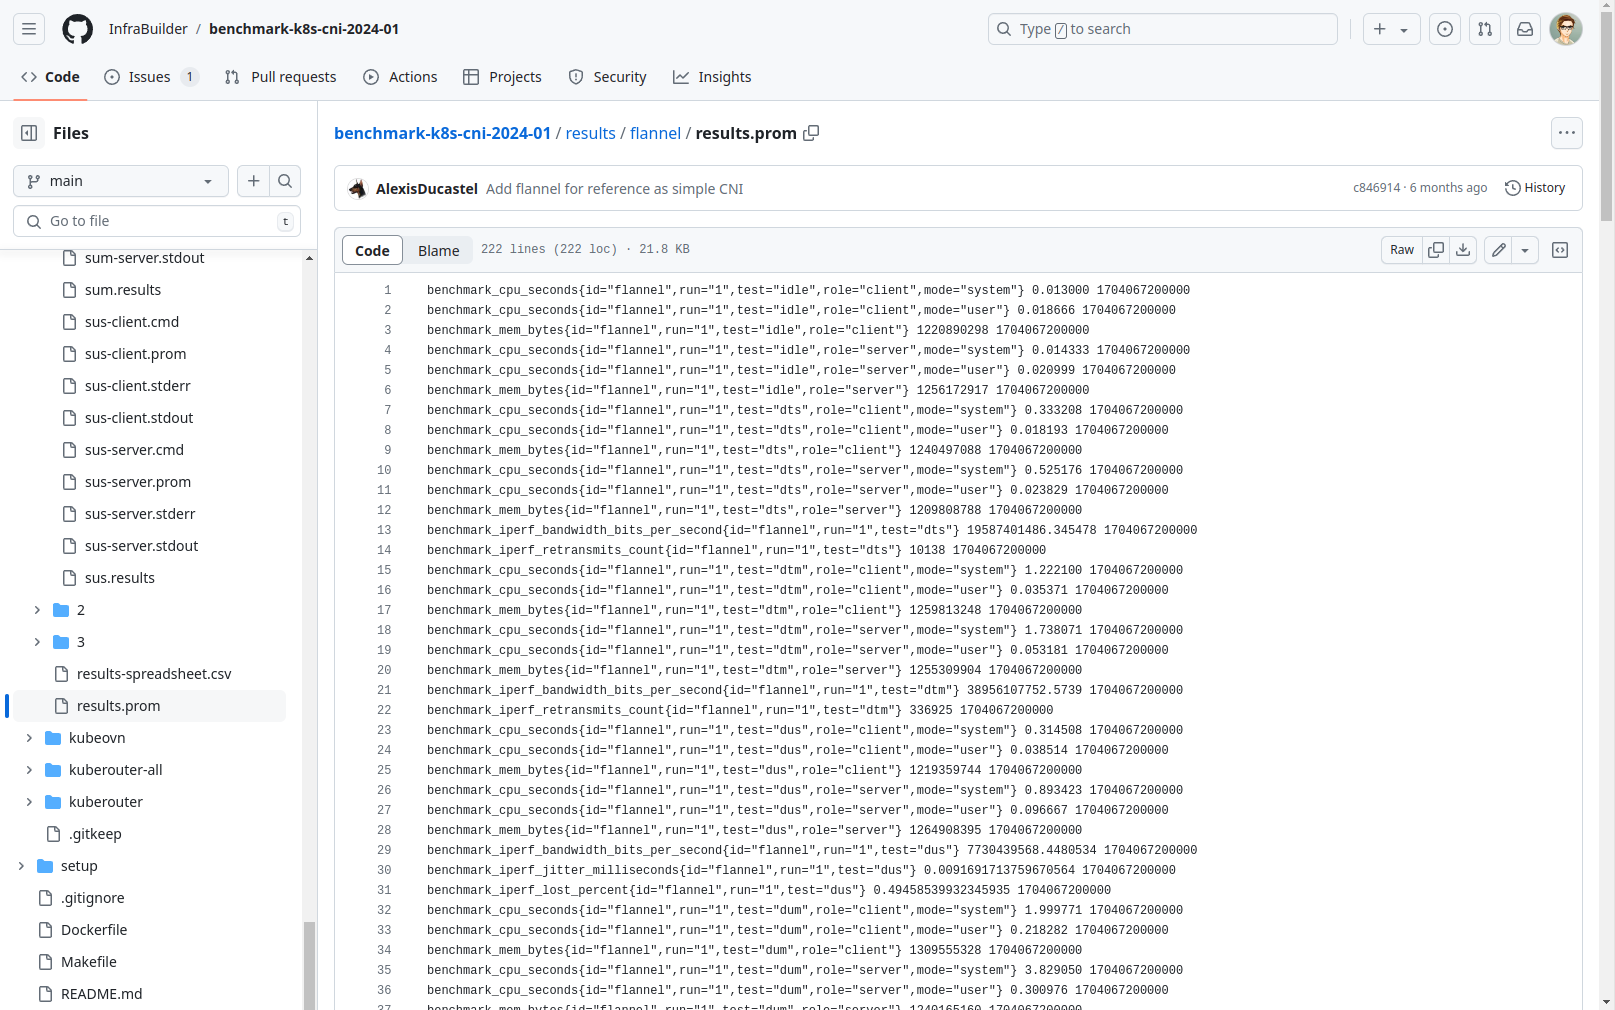
\includegraphics[width=\linewidth]{images/flannel-prom.png}
\label{fig:flannel-prom}
\end{figure}

The original raw data for 2024 is formatted as \href{https://prometheus.io/docs/concepts/metric_types/#gauge}{Prometheus gauges}, also split by CNI.

\subsubsection{2020 and 2021 Header}

From the overall aggregated result spreadsheet, we added the following headers to the TSV Files and converted them to CSV format:

\begin{itemize}
    \item smem - "Server Memory (MB)"
    \item scpu - "Server CPU (\%)"
    \item cmem - "Client Memory (MB)"
    \item ccpu - "Client CPU (\%)"
    \item tcpbw - "TCP Pod to Pod Bandwidth (Mbit/s)"
    \item tcpsm - "Server Memory (MB)"
    \item tcpsc - "Server CPU (\%)"
    \item tcpcm - "Client Memory (MB)"
    \item tcpcc - "Client CPU (\%)"
    \item udpbw - "UDP Pod to Pod Bandwidth (Mbit/s)"
    \item udpsm - "Server Memory (MB)"
    \item udpsc - "Server CPU (\%)"
    \item udpcm - "Client Memory (MB)"
    \item udpcc - "Client CPU (\%)"
    \item tcpebw - "TCP Pod to Service Bandwidth (Mbit/s)"
    \item tcpesm - "Server Memory (MB)"
    \item tcpesc - "Server CPU (\%)"
    \item tcpecm - "Client Memory (MB)"
    \item tcpecc - "Client CPU (\%)"
    \item udpebw - "UDP Pod to Service Bandwidth (Mbit/s)"
    \item udpesm - "Server Memory (MB)"
    \item udpesc - "Server CPU (\%)"
    \item udpecm - "Client Memory (MB)"
    \item udpecc - "Client CPU (\%)"
\end{itemize}

We also removed the discovered MTU size from the measurements, as it was a constant value and was also not present in the 2024 data.

\subsubsection{2024 Data Transformation}

The 2024 data format was vastly different, and we decided to convert the Prometheus gauges into CSV for easier handling. The 2024 data also had many more data points, so we mapped the gauges to the most appropriate fields and adjusted the scale where necessary (e.g., Bytes to Megabytes).

\begin{itemize}
    \item smem - "benchmark\_mem\_bytes - server - idle"
    \item scpu - "benchmark\_cpu\_seconds - server - idle"
    \item cmem - "benchmark\_mem\_bytes - client - idle"
    \item ccpu - "benchmark\_cpu\_seconds - client - idle"
    \item tcpbw - "benchmark\_iperf\_bandwidth\_bits\_per\_second - dts"
    \item tcpsm - "benchmark\_mem\_bytes - server - dts"
    \item tcpsc - "benchmark\_cpu\_seconds - server - dts"
    \item tcpcm - "benchmark\_mem\_bytes - client - dts"
    \item tcpcc - "benchmark\_cpu\_seconds - client - dts"
    \item udpbw - "benchmark\_iperf\_bandwidth\_bits\_per\_second - dus"
    \item udpsm - "benchmark\_mem\_bytes - server - dus"
    \item udpsc - "benchmark\_cpu\_seconds - server - dus"
    \item udpcm - "benchmark\_mem\_bytes - client - dus"
    \item udpcc - "benchmark\_mem\_bytes - client - dus"
    \item tcpebw - "benchmark\_iperf\_bandwidth\_bits\_per\_second - sts"
    \item tcpesm - "benchmark\_mem\_bytes - server - sts"
    \item tcpesc - "benchmark\_cpu\_seconds - server - sts"
    \item tcpecm - "benchmark\_mem\_bytes - client - sts"
    \item tcpecc - "benchmark\_cpu\_seconds - client - sts"
    \item udpebw - "benchmark\_iperf\_bandwidth\_bits\_per\_second - sus"
    \item udpesm - "benchmark\_mem\_bytes - server - sus"
    \item udpesc - "benchmark\_cpu\_seconds - server - sus"
    \item udpecm - "benchmark\_mem\_bytes - client - sus"
    \item udpecc - "benchmark\_mem\_bytes - client - sus"
\end{itemize}

\subsection{What's Not in the Data}

The benchmark data was recorded with the author's \href{https://github.com/InfraBuilder/k8s-bench-suite}{k8s-bench-suite}.

The 2020 \href{https://github.com/InfraBuilder/benchmark-k8s-cni-2020-08/blob/master/PROTOCOL.md}{setup} was three \href{https://www.supermicro.com/en/}{Supermicro} bare-metal servers connected through a Supermicro 10Gbit switch, running \href{https://ubuntu.com/server}{Ubuntu} 18.04 LTS and Kubernetes 1.19.0.

2020 CNI Versions:
\begin{itemize}
    \item Flannel: v0.12.0
    \item Calico: v3.16.1
    \item Canal: v3.16.1
    \item Cilium: v1.8.2
\end{itemize}

The 2021 \href{https://github.com/InfraBuilder/benchmark-k8s-cni-2021-05/blob/main/PROTOCOL.md}{setup} was three Supermicro bare-metal servers connected through a Supermicro 10Gbit switch, running Ubuntu 20.04 LTS and Kubernetes 1.21.0.

2021 CNI Versions:
\begin{itemize}
    \item Flannel: v0.15.1
    \item Calico: v3.19.2
    \item Canal: v3.19.2
    \item Cilium: v1.11.2
\end{itemize}

For 2024, three Supermicro bare-metal servers were connected through a Supermicro 40Gbit switch, running Ubuntu 22.04 LTS and Kubernetes 1.26.12.\footnote{See \textit{Ducastel, A. (2024)}: Benchmark results of Kubernetes network plugins. \cite{originalArticle}}

2024 CNI Versions:
\begin{itemize}
    \item Flannel: v0.24.3
    \item Calico: v3.27.2
    \item Canal: v3.27.2
    \item Cilium: v1.15.2
\end{itemize}

\subsection{Data Exploration}

We will analyze the data sets using the methods of Exploratory Data Analysis (EDA).

John Tukey has promoted EDA since 1977 to encourage data scientists to explore data and formulate hypotheses that could lead to new data collection and experiments.\footnote{See \textit{Tukey, J.W. (1977)}: Exploratory data analysis. \cite{exploratoryDA}}

EDA uses statistical methods to analyze and visualize the data, understand key characteristics, and identify patterns and relationships. We will not use the data to predict performance gains in future releases of the CNIs or through improved network speeds.

\subsection{Tools}

We performed most of the initial data wrangling with \href{https://www.gnu.org/software/bash/}{Bash}, \href{https://pubs.opengroup.org/onlinepubs/9699919799/utilities/vi.html}{vi}, and \href{https://www.microsoft.com/en-us/microsoft-365/excel}{Microsoft Excel}.

For the subsequent data exploration, we used \href{https://www.r-project.org/}{R} and \href{https://posit.co/download/rstudio-desktop/}{RStudio}.


%
%	Theorieteil
%

\pagebreak
\section{Data Exploration}

\onehalfspacing

\subsection{2020}

\subsubsection{Flannel}

\subsubsection{Calico}

\subsubsection{Canal}

\subsubsection{Cilium}

\subsection{2021}

\subsubsection{Flannel}

\subsubsection{Calico}

\subsubsection{Canal}

\subsubsection{Cilium}

\subsection{2024}

\subsubsection{Flannel}

\subsubsection{Calico}

\subsubsection{Canal}

\subsubsection{Cilium}


%
%	Praxisbezug
%

\pagebreak
\section{Data Analysis}

\onehalfspacing

\subsection{Performance Considerations}

\subsection{Server CPU Usage}

\begin{table}[H]
\caption{Median Server CPU Usage}
\begin{tabular}{|c | c | c | c | c|} 
 \hline
 Year & Flannel & Calico & Canal & Cilium \\
 \hline\hline
 2020 & 5.05 & 6.44 & 6.69 & 13.22 \\ 
 \hline
 2021 & 5.01 & 6.36 & 6.66 & 12.77 \\
 \hline
 2024 & 5.05 & 5.44 & 5.64 & 6.15 \\
 \hline
\end{tabular}
\label{tab:cpu}
\end{table}

\subsection{Server Memory Usage}

\begin{table}[H]
\caption{Median Server Memory Consumption}
\begin{tabular}{|c | c | c | c | c|} 
 \hline
 Year & Flannel & Calico & Canal & Cilium \\
 \hline\hline
 2020 & 590 & 659 & 655 & 866 \\ 
 \hline
 2021 & 590 & 661 & 659 & 867 \\
 \hline
 2024 & 1175 & 1420 & 1285 & 1521 \\
 \hline
\end{tabular}
\label{tab:mem}
\end{table}

\subsection{Pod-to-Pod Bandwidth}

\begin{table}[H]
\caption{Median Pod-to-Pod Bandwidth}
\begin{tabular}{|c | c | c | c | c|} 
 \hline
 Year & Flannel & Calico & Canal & Cilium \\
 \hline\hline
 2020 & 9705 & 8882 & 8634 & 9475 \\ 
 \hline
 2021 & 9695 & 8876 & 8612 & 9444 \\
 \hline
 2024 & 19166 & 18571 & 16842 & 20709 \\
 \hline
\end{tabular}
\label{tab:p2pbw}
\end{table}

\subsection{Pod-to-Server Bandwidth}

\begin{table}[H]
\caption{Median Pod-to-Server Bandwidth}
\begin{tabular}{|c | c | c | c | c|} 
 \hline
 Year & Flannel & Calico & Canal & Cilium \\
 \hline\hline
 2020 & 9828 & 8675 & 8576 & 9673 \\ 
 \hline
 2021 & 9825 & 8763 & 8579 & 9679 \\
 \hline
 2024 & 19942 & 19263 & 16328 & 21758 \\
 \hline
\end{tabular}
\label{tab:p2ebw}
\end{table}

\subsection{Results}

For real,\footnote{See \textit{Kelly, J. (2024)}: Gen-Z Slang Is Revolutionizing Work Jargon. \cite{genzSlang}} I think Flannel is the next option

\subsection{Outlook}


%
%	Fazit
%

\pagebreak
\section{Summary}

\onehalfspacing

The data analysis showed marked improvements in Kubernetes networking performance over the last couple of years. We saw performance improvements across the board for all four CNIs included with SUSE's Rancher Kubernetes Engine.

The power is in the data—we were able to identify Flannel and Cilium as the two CNIs that will deliver the best performance and recommend them for future cluster configurations.

Cilium is the most promising new development in Kubernetes networking, and the venerable Flannel is holding up well, delivering similar performance with a smaller footprint and a smaller feature set.

We were merely able to scratch the surface with this secondary analysis, but I do hope that you will find at least some valuable insights and pointers to start with. A big shoutout to Alexis Duscatel of infraBuilder; none of this would have been possible without their excellent work.

To quote Toshinori Yagi: “Next, it’s your turn.”\footnote{\textit{Crunchyroll (2024)}: 40 My Hero Academia Quotes Worth Remembering. \cite{mhaQuotes}} - go and create your own cluster!

Happy Ranching!


% Literaturverzeichnis
\cleardoublepage
\raggedright
\bibliographystyle{IEEEtranS}	% ieeetran verwenden, damit auch URLs angezeigt werden
\bibliography{seminar-lit}

\cleardoublepage
\justify
%
%	Ehrenwoertliche Erklaerung
%

\pagebreak

\pagenumbering{gobble} % Keine Seitenzahlen mehr
\onehalfspacing

%-----------------------------------
% Ehrenwoertliche Erklärung
%-----------------------------------
\section*{Declaration in lieu of oath}

\par\medskip

With this, I declare that I produced the submitted paper without any other party's assistance and without using any unauthorized aids. In particular, I have marked all passages reproduced verbatim or near-verbatim from publications as quotations. Also, I declare that the submitted print version of this thesis is identical to its digital version. Further, I have never introduced this thesis to any examination board in its present form or in any other similar version. I herewith agree that you may publish this thesis. I herewith consent to you uploading this thesis to an external contractor's server to submit it to the contractor's plagiarism detection systems. Uploading this thesis to send it to plagiarism detection systems is not a form of publication.

\par\medskip
\par\medskip

\vspace{5cm}

\begin{table}[H]
	\begin{tabular*}{\textwidth}{c @{\extracolsep{\fill}} ccccc}
		Cologne, \the\month/\the\day/\the\year \\
		\rule[0.5ex]{12em}{0.55pt} & \rule[0.5ex]{12em}{0.55pt} \\
		(Location, Date) & (Signature)
	\end{tabular*}
\end{table}


\end{document}
